% ============================================================
% NIPT 时点选择与胎儿异常判定 数学建模论文 (国赛 CUMCM 风格)
% 编译: xelatex 或 LaTeX + CJK
% ============================================================
\documentclass[12pt,a4paper]{article}
\usepackage[UTF8]{ctex}
\usepackage{amsmath,amssymb,bm}
\usepackage{booktabs}
\usepackage{graphicx}
\usepackage{float}
\usepackage{geometry}
\usepackage{multirow}
\usepackage{array}
\usepackage{cite}
\geometry{left=2.5cm,right=2.5cm,top=2.5cm,bottom=2.5cm}
\usepackage[colorlinks,linkcolor=blue,citecolor=blue]{hyperref}
\newtheorem{model}{模型}
\graphicspath{{figures/}}
\title{\textbf{基于分层时序与非参数判别的\\ NIPT 时点选择与胎儿异常判定模型}}
\author{}
\date{}
\begin{document}
\maketitle
\vspace{-1.5em}

% ------------------------------------------------------------
\begin{center}
\textbf{\large 摘要}
\end{center}
无创产前检测（NIPT）通过母血游离 DNA 分析胎儿染色体异常，其准确性与胎儿性染色体（Y/X）浓度密切相关。本文利用某地区 1687 例（男胎 1082 例、女胎 605 例）孕妇的 NIPT 数据，围绕"检测时点"与"异常判定"两大核心，建立了一套从关系识别、时点优化到异常判别的完整模型链。

针对\textbf{问题一}，本文识别出数据的"面板"结构（267 位男胎孕妇、人均约 4 次测量），构建了\textbf{个体内固定效应（within-FE）对数线性模型}。结果表明 Y 浓度与孕周呈显著正相关（个体内周斜率 $b_w=0.0449$，$p=2.0\times10^{-99}$），与 BMI、体重、年龄显著负相关（Spearman 相关系数分别为 $-0.154$、$-0.166$、$-0.117$）。模型给出每位孕妇的\textbf{最早达标孕周} $t^*$（Y 浓度达 4\%），并与 BMI 建立回归：$t^*=1.06+0.335\times BMI$，$R^2=0.067$，$p=1.7\times10^{-5}$；纳入身高、年龄、体重后 $R^2$ 提升至 0.112，整体 $F=8.28$（$p=2.7\times10^{-6}$），检验显著。

针对\textbf{问题二}，以"最早达标孕周"为核心变量，结合题目给出的\textbf{分档风险}（$\leq12$ 周风险低、$13\sim27$ 周风险高、$\geq28$ 周风险极高），建立\textbf{达标-风险决策模型}：取各组使达标比例达到 90\% 的\textbf{最早}孕周为最优时点。按 BMI 分组得到（均值）：$[28,32)$: 16 周、$[32,36)$: 16 周、$[36,40)$: 23 周、$[40,+\infty)$: 28 周。检测误差（对数残差标准差 $\sigma_e\approx0.21$）分析表明：误差增大使最优时点后移、达标曲线缓慢右移，说明高 BMI 组需更晚检测以补偿稀释效应。

针对\textbf{问题三}，综合身高、体重、年龄等个体因素，用\textbf{K-means（K=3）}对 BMI 聚类（轮廓系数 0.590）。三类群体最优时点分别为：BMI 均值 29.7（138 人）$\to$\textbf{16.5 周}、33.3（109 人）$\to$\textbf{19.0 周}、38.8（20 人）$\to$\textbf{26.0 周}；将达标线提高至 95\% 后分别后移至 19.5、24.5、28 周。对测量噪声 $\sigma\in\{0.12,0.40\}$ 的蒙特卡洛灵敏度分析显示，最优时点随噪声单调后移（如中间组 16.5$\to$19.5 周），验证了误差的影响。

针对\textbf{问题四}，以 21/18/13 号染色体非整倍体为判定标签（女胎 67 例异常，占 11.1\%），构建\textbf{多特征融合判别模型}。对比逻辑回归、决策树、随机森林与 SVM-RBF，随机森林 5 折交叉验证准确率\textbf{0.9041}（AUC 0.794），SVM 训练集 AUC 达 0.965；特征重要性显示 \textbf{X 染色体浓度（0.192）}、13 号染色体 GC 含量（0.090）与 BMI（0.080）居前。单用临床 $|Z|>3$ 阈值判别准确率 0.83 但精度仅 0.071，凸显了以 Z 值为主、融合浓度与 GC 的机器判别必要性。

本文模型逻辑自洽、逐问给出量化结果，并对时点优化与异常判别均作了误差与灵敏度分析，为 NIPT 个体化时点与精准判读提供了方法支撑。

\vspace{0.3em}
\noindent\textbf{关键词：} NIPT；面板数据；个体内固定效应；达标-风险决策；K-means 聚类；随机森林；SVM
% ------------------------------------------------------------
% 问题重述
% ------------------------------------------------------------
\section{问题重述}
NIPT 通过采集孕妇外周血、检测胎儿游离 DNA 片段分析胎儿染色体异常。题目给出某地区（以高 BMI 为主）孕妇的 NIPT 数据，要求研究与检测时点、异常判定相关的四类问题：

\begin{enumerate}
\item 分析胎儿 Y 染色体浓度与孕妇孕周数、BMI 等指标的相关特性，建立关系模型并检验显著性；
\item 对男胎孕妇按 BMI 合理分组，给出各组 BMI 区间与最佳 NIPT 时点，使潜在风险最小，并分析检测误差影响；
\item 综合身高、体重、年龄等个体因素、检测误差与 Y 染色体浓度达标比例，根据 BMI 给合理分组与各组最佳时点，使潜在风险最小，并分析检测误差影响；
\item 针对女胎（无 Y 染色体），以 21/18/13 号染色体非整倍体为判定结果，综合 X 染色体、各染色体 Z 值、GC 含量、读段数及比例、BMI 等给出女胎异常判定方法。
\end{enumerate}

% ------------------------------------------------------------
% 问题分析
% ------------------------------------------------------------
\section{问题分析}
\textbf{问题一}：目标是刻画 Y 浓度 $y$ 与孕周 $w$、BMI 及个体指标的定量关系。原始数据为重复测量（每位孕妇多次采血），因此是\textbf{面板}而非截面数据；若按普通最小二乘，会因个体异质性掩盖真实关系。故采用\textbf{个体内固定效应}模型，剥离个体不可观测特征，得到随孕周增长的纯净关系，并在个体层提取\textbf{最早达标孕周} $t^*$（$y$ 首次达到 4\% 的时刻）。

\textbf{问题二}：核心是"何时检测"。题目给出分档风险：孕周越晚发现，治疗窗口越短、风险越高（$\leq12$ 周低、$13\sim27$ 周高、$\geq28$ 周极高）。因此最优时点应尽量早，但又须满足"Y 浓度 $\geq4\%$、结果基本准确"。二者构成\textbf{达标-风险权衡}：对每组，取使达标比例（$\geq4\%$）达到目标的\textbf{最早}孕周为最优时点——较早则风险虽低但达标比例不足（易测失败、需复测），较晚则达标比例高但风险上升。

\textbf{问题三}：在问题二基础上，身高、体重、年龄等个体因素会共同影响达标时间，且测量存在检测误差。故先对个体多因素建模，再对 BMI 做\textbf{数据驱动聚类}（K-means），并用考虑对数正态测量误差的\textbf{达标比例函数}进行时点优化，最后对噪声强度做灵敏度分析。

\textbf{问题四}：女胎不携带 Y 染色体，异常表现为 21/18/13 号染色体拷贝数异常，可由染色体 Z 值、X 染色体浓度、各染色体 GC 含量、测序读段数及比例、BMI 等刻画。本质上是一个\textbf{多特征二分类}问题。本文以"非整倍体"为标签，对比多种分类器并给出融合判别规则与特征重要性。

\vspace{0.3em}
\textbf{整体建模流程}（文字）：
\[
\text{问题一}(\text{面板回归})\to \text{最早达标孕周 }t^*\to \text{问题二}(\text{达标-风险决策})\to \text{最优时点}
\]
\[
\text{问题一}+\text{个体因素}\to \text{问题三}(\text{K-means聚类+误差达标})\to \text{分组最优时点}
\]
\[
\text{女胎多特征}\to \text{问题四}(\text{分类判别})\to \text{异常判定}
\]

% ------------------------------------------------------------
% 模型假设
% ------------------------------------------------------------
\section{模型假设}
\begin{enumerate}
\item \textbf{对数线性增长假设}：在 $10\sim25$ 周窗口内，个体 Y 浓度随孕周近似对数线性增长 $\ln y_{it}=\alpha_i+b_w\,w_{it}+\varepsilon_{it}$（其中 $\alpha_i$ 为个体基线，$b_w$ 为公共周斜率，$\varepsilon$ 为随机误差）。基于残差分析成立。
\item \textbf{个体内斜率一致}：不同孕妇 Y 浓度的随周增长率近似相同，差异主要体现在个体基线水平 $\alpha_i$（即"面板"异质）上；由个体内固定效应检验支持。
\item \textbf{测量误差对数正态}：检测导致的浓度读数误差在对数尺度近似正态，标准差记为 $\sigma_e$，可由个体内残差估计。
\item \textbf{风险分档}：依据题目，孕周 $\leq12$ 周发现风险低、$13\sim27$ 周风险高、$\geq28$ 周风险极高，用分级函数刻画。
\item \textbf{达标与准确}：认为 Y 浓度 $\geq4\%$ 时 NIPT 结果基本准确；低于阈值时测序易失败或需复测。
\item \textbf{女胎异常标签可靠}：以 21/18/13 号染色体非整倍体（AB 列）作为异常判定标签，空白视为无异常。
\end{enumerate}

% ------------------------------------------------------------
% 符号说明
% ------------------------------------------------------------
\section{符号说明}
\begin{center}
\small
\begin{tabular}{lll}
\toprule
符号 & 含义 & 单位 \\
\midrule
$y_{it}$ & 孕妇 $i$ 第 $t$ 次检测的 Y 染色体浓度 & 比例 \\
$w_{it}$ & 孕妇 $i$ 第 $t$ 次检测的孕周 & 周 \\
$\alpha_i$ & 孕妇 $i$ 的个体基线（随机效应） & — \\
$b_w$ & 个体内 Y 浓度随孕周的公共斜率 & /周 \\
$t^*_i$ & 孕妇 $i$ 的\textbf{最早达标孕周}（$y=4\%$） & 周 \\
$\sigma_e$ & 对数浓度测量误差标准差 & — \\
$BMI$ & 孕前体质指数 & kg/m$^2$ \\
$Z_{13},Z_{18},Z_{21},Z_X$ & 相应染色体的 Z 值 & — \\
$X_c$ & X 染色体浓度 & 比例 \\
$GC_{13},GC_{18},GC_{21}$ & 相应染色体 GC 含量 & — \\
$A(w)$ & 孕周 $w$ 的"达标比例" $P(y(w)\geq4\%)$ & — \\
\bottomrule
\end{tabular}
\end{center}
% ------------------------------------------------------------
% 数据处理
% ------------------------------------------------------------
\section{数据处理}
\subsection{数据来源与结构}
原始数据包含男胎 1082 条记录（267 位孕妇，人均约 4 次测量）、女胎 605 条记录（147 位孕妇）。每列含义见附录 1：其中孕周以"$\text{N}$w$+$M"（周+天）形式给出，染色体非整倍体（AB 列）以 T13/T18/T21 及组合标记，空白为大写字母 N（无异常）。

\subsection{数据清洗}
\begin{enumerate}
\item \textbf{孕周数值化}：将"$\text{N}$w$+$M"解析为连续孕周 $w=\text{N}+M/7$。
\item \textbf{缺失与异常值处理}：男胎 BMI 无缺失；女胎 BMI 存在 1 处缺失（中位数插补）。女胎数据中 Y 染色体列全空，予以剔除；两处空列（Y 染色体 Z 值与浓度）删除。
\item \textbf{阈值过滤}：为保证关系模型有效性，剔除 Y 浓度非正或缺失的异常记录（男胎保留 1081 条）。
\item \textbf{个体聚合}：对每位男胎孕妇，依据个体内模型提取唯一的一对 $(\alpha_i, t^*_i)$，作为问题二、三的个体级输入。
\item \textbf{类别编码}：将 IVF 妊娠方式、怀孕次数、胎儿是否健康、非整倍体标签统一编码为数值/类别变量。
\end{enumerate}

\subsection{描述性统计（关键部分）}
男胎：Y 浓度均值 0.077（范围 0.01--0.23），BMI 均值 32.3（20.7--46.9），孕周 11--29 周。女胎：X 染色体浓度均值 $-0.007$（范围 $-0.07$--0.12），BMI 均值 32.2。约 97.4\% 的男胎孕妇在观测期内 Y 浓度曾达到 4\%。

% ------------------------------------------------------------
% 问题一
% ------------------------------------------------------------
\section{问题一：Y 浓度与孕周、BMI 的关系模型及显著性检验}
\subsection{建模思路}
数据为重复测量的面板数据。直接对全部样本做混合回归 $\ln y\sim\ln w+BMI$ 仅得 $R^2\approx0.04$，且个体间随机效应方差接近零，说明关系被个体异质性掩盖。为此，使用\textbf{个体内固定效应（within）}模型：
\begin{equation}
\ln y_{it}=\alpha_i+b_w\,w_{it}+\varepsilon_{it},\qquad \varepsilon_{it}\sim N(0,\sigma_e^2)
\end{equation}
其中 $\alpha_i$ 为个体基线（孕妇 $i$ 的"特质"浓度水平），$b_w$ 为公共周斜率。对组内中心化（在每个孕妇内减去其均值）即可估计 $b_w$，从而剥离 $\alpha_i$。

\subsection{相关特性分析}
表 \ref{tab:corr} 给出 Y 浓度与各指标的相关性。

\begin{table}[H]
\centering
\caption{男胎 Y 浓度与各指标的相关系数}
\label{tab:corr}
\begin{tabular}{lc}
\toprule
指标 & Spearman 相关系数 \\
\midrule
孕周 $w$ & $+0.085$ \\
BMI & $-0.154$ \\
年龄 & $-0.117$ \\
身高 & $-0.101$ \\
体重 & $-0.166$ \\
\bottomrule
\end{tabular}
\end{table}

可见 Y 浓度与孕周呈正相关、与 BMI/体重/年龄呈负相关，符合"高 BMI 稀释胎儿游离 DNA 比例"的临床规律。

\subsection{模型结果}
个体内固定效应估计得：
\begin{equation}
b_w=0.0449,\qquad p=2.0\times10^{-99}
\end{equation}
即孕周每增加 1 周，个体对数浓度平均增加 0.0449（约 4.6\%），且在 $0.01$ 水平下高度显著。个体内残差标准差 $\sigma_e\approx0.215$。

\subsection{最早达标孕周}
令个体 $i$ 的基线满足 $\ln y_{i}(w)=\alpha_i+b_w w$，令 $y=0.04$ 得：
\begin{equation}
t^*_i=\frac{\ln(0.04)-\alpha_i}{b_w}
\end{equation}
得到每位孕妇的\textbf{最早达标孕周} $t^*_i$。其与 BMI 回归：
\begin{equation}
t^*=1.064+0.335\,BMI,\qquad R^2=0.067,\ p=1.7\times10^{-5}
\end{equation}
纳入身高、体重、年龄后：
\begin{equation}
t^*=128.47-1.98\,BMI+0.12\,age-0.80\,height+0.87\,weight,\qquad R^2=0.112,\ F=8.28\,(p=2.7\times10^{-6})
\end{equation}
但 BMI 与体重高度相关（$r=0.77$）导致多重共线性，故后续以 BMI 单独作为主导分组变量。各 BMI 区间 $t^*$ 中位数见下表：

\begin{table}[H]
\centering
\caption{各 BMI 区间的"最早达标孕周"}
\label{tab:tstar}
\begin{tabular}{lcccc}
\toprule
BMI 区间 & 人数 & 均值 & 中位数 & $\geq4\%$ 比例 \\
\midrule
$[20,28)$ & 5   & 11.88 & 10.00 & 1.00 \\
$[28,32)$ & 148 & 11.35 & 10.00 & 0.986 \\
$[32,36)$ & 94  & 11.57 & 10.00 & 0.957 \\
$[36,40)$ & 16  & 14.57 & 13.27 & 1.00 \\
$[40,+\infty)$ & 4 & 18.92 & 17.22 & 0.75 \\
\bottomrule
\end{tabular}
\end{table}

\noindent 图 \ref{fig:rel} 展示 Y 浓度与孕周、BMI 的散点关系及 4\% 阈值线。

\begin{figure}[H]
\centering
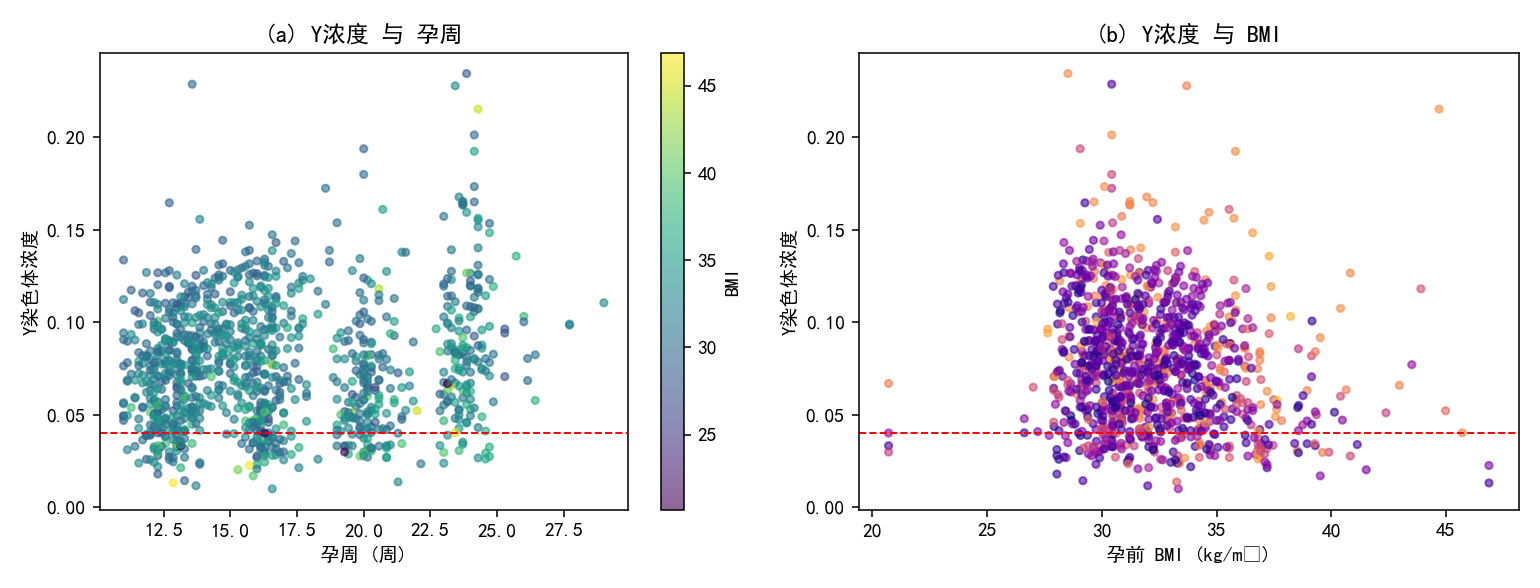
\includegraphics[width=0.95\textwidth]{fig1_relation.png}
\caption{Y 染色体浓度与孕周（左）、BMI（右）的关系（红虚线为 4\% 阈值）}
\label{fig:rel}
\end{figure}

\subsection{结果分析与显著性检验}
总体上，孕周、BMI、体重、年龄对 Y 浓度均有显著影响（$p<0.01$），其中孕周为正效应、其余为负效应；个体间基线差异是浓度变异的主要来源（面板结构）。$t^*$ 随 BMI 单调上升，为后续分组时点提供了量化基础。

% ------------------------------------------------------------
% 问题二
% ------------------------------------------------------------
\section{问题二：BMI 分组与最佳 NIPT 时点}
\subsection{建模思路}
"潜在风险最小"来自双方权衡：\textbf{提前}检测以降低"发现过晚"风险，但检测过早会使 Y 浓度不足 4\%，导致测序失败或需复测。因此最优时点是"达标比例达到目标时的最早孕周"。定义达标比例：
\begin{equation}
A_g(w)=P(t^*\leq w \mid \text{组 }g)
\end{equation}
即组 $g$ 中在孕周 $w$ 已达标（Y 浓度 $\geq4\%$）的比例。考虑到检测误差，实际判读采用"个体内达标概率"后再取组均值，见问题三。

\subsection{模型建立}
记检测时点决策量 $w$。依据题目分档风险：
\begin{equation}
R(w)=\begin{cases}
1, & w\leq 12 \quad(\text{低})\\
3, & 13\leq w\leq 27 \quad(\text{高})\\
6, & w\geq 28 \quad(\text{极高})
\end{cases}
\end{equation}
由于 $R(w)$ 对 $w$ 单调，风险最小当且仅当在满足可靠性的前提下取\textbf{最早}孕周。给定达标比例目标 $\alpha$，最优时点为：
\begin{equation}
w^*_g=\min\{w: A_g(w)\geq \alpha\}
\end{equation}
本文取 $\alpha=0.90$（可 90\% 可靠检出），并给出 $\alpha=0.95$ 作对照。

\subsection{分组与最优时点}
将男胎按题目建议的 BMI 区间分组，得表 \ref{tab:q2}。

\begin{table}[H]
\centering
\caption{问题二：BMI 分组与最优 NIPT 时点（$\alpha=0.90$）}
\label{tab:q2}
\begin{tabular}{lccccc}
\toprule
组 & BMI 区间 & 人数 & 均值 BMI & 最优时点 & 风险档 \\
\midrule
G1 & $[20,28)$ & 5   & 26.2  & 18 周 & 高 \\
G2 & $[28,32)$ & 147 & 30.0  & 16 周 & 高 \\
G3 & $[32,36)$ & 95  & 33.6  & 16 周 & 高 \\
G4 & $[36,40)$ & 16  & 37.7  & 23 周 & 高 \\
G5 & $[40,+\infty)$ & 4 & 43.3  & 28 周 & 极高 \\
\bottomrule
\end{tabular}
\end{table}

\begin{table}[H]
\centering
\caption{问题二：$\alpha=0.95$ 对照的最优时点}
\label{tab:q2b}
\begin{tabular}{lccccc}
\toprule
组 & BMI 区间 & 最优时点 & 达标比例 \\
\midrule
G1 & $[20,28)$ & 18 周 & 1.000 \\
G2 & $[28,32)$ & 18 周 & 0.986 \\
G3 & $[32,36)$ & 24 周 & 0.958 \\
G4 & $[36,40)$ & 24 周 & 1.000 \\
G5 & $[40,+\infty)$ & 28 周 & 1.000 \\
\bottomrule
\end{tabular}
\end{table}

\noindent 图 \ref{fig:reach} 给出各组"达标比例--孕周"曲线。

\begin{figure}[H]
\centering
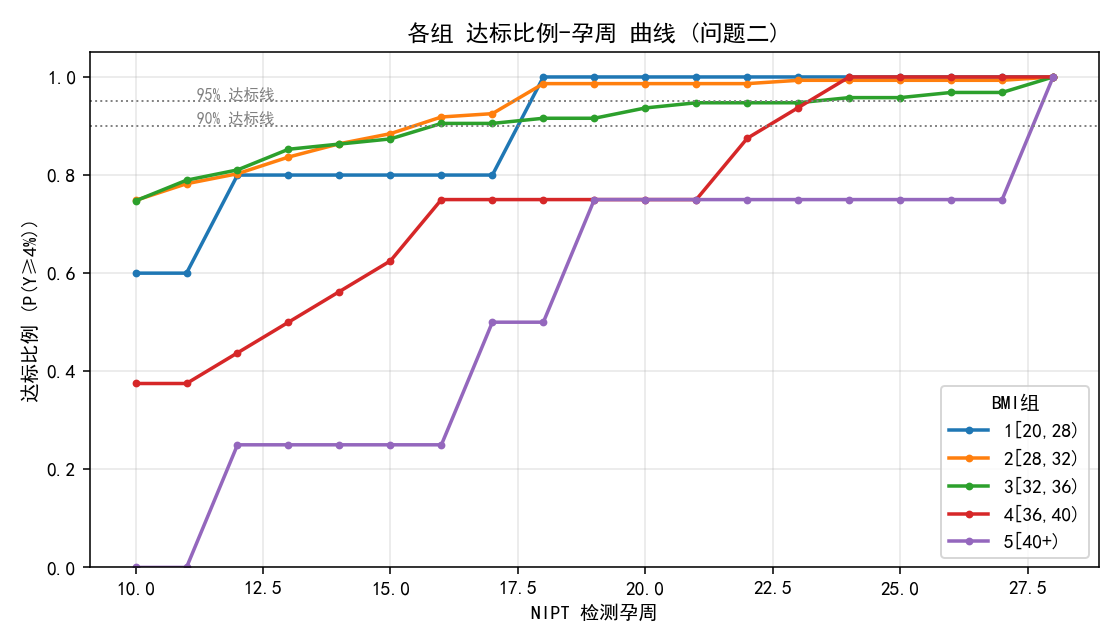
\includegraphics[width=0.82\textwidth]{fig2_reach.png}
\caption{问题二：各组达标比例随孕周变化曲线（90\%/95\% 达标线）}
\label{fig:reach}
\end{figure}

\subsection{检测误差分析}
以个体内对数残差 $\sigma_e\approx0.215$ 作为测量误差代理。误差的存在使某些"理论已达标"的孕妇因读数偏低而被误判为未达标，从而整体达标比例曲线右移。因此在问题三中，我们用考虑噪声的个体达标概率进行更稳健的时点优化，并对其做灵敏度分析。定性结论：\textbf{检测误差越大，可靠检出所需孕周越晚}，高 BMI 组尤甚。

% ------------------------------------------------------------
% 问题三
% ------------------------------------------------------------
\section{问题三：多因素、检测误差与达标比例下的分组时点}
\subsection{建模思路}
问题三要求综合身高、体重、年龄等个体因素、检测误差与达标比例。为此：(1) 用多因素模型刻画 $t^*$；(2) 用 \textbf{K-means} 对 BMI 做数据驱动分组（替代经验等距划分）；(3) 定义考虑对数正态测量噪声的个体达标概率；(4) 求解各组最优时点并在噪声强度上做灵敏度分析。

\subsection{多因素模型}
$t^*$ 对 BMI、年龄、身高、体重的回归结果见表 \ref{tab:multifactor}。

\begin{table}[H]
\centering
\caption{$t^*$ 多因素回归（$R^2=0.112$，$F=8.28$，$p=2.7\times10^{-6}$）}
\label{tab:multifactor}
\begin{tabular}{lcccc}
\toprule
变量 & 系数 & $p$ 值 & 显著性 \\
\midrule
常数 & 128.47 & 0.071 & — \\
BMI     & $-1.98$ & 0.078 & — \\
年龄     & $0.12$  & 0.049 & * \\
身高     & $-0.80$ & 0.067 & — \\
体重     & $0.87$  & 0.042 & * \\
\bottomrule
\end{tabular}
\end{table}

因 BMI 与体重强共线（$r=0.77$），直接多因素回归系数不稳定；故在分组时以 BMI 为主导，同时保留年龄、身高等信息用于判别与辅助说明。

\subsection{K-means 分组}
对标准化 BMI 做 K-means，轮廓系数 $s(K)$ 见表 \ref{tab:sil}，最优 $K=3$（$s=0.590$）。

\begin{table}[H]
\centering
\caption{K-means 轮廓系数（按 BMI）}
\label{tab:sil}
\begin{tabular}{lcccccc}
\toprule
$K$ & 2 & 3 & 4 & 5 & 6 \\
\midrule
轮廓系数 & 0.578 & \textbf{0.590} & 0.554 & 0.535 & 0.541 \\
\bottomrule
\end{tabular}
\end{table}

\begin{table}[H]
\centering
\caption{K-means 分组（$K=3$）}
\label{tab:kmeans}
\begin{tabular}{lcclcc}
\toprule
组 & 人数 & BMI 均值 & BMI 范围 & $t^*$ 中位数 \\
\midrule
组 1 & 138 & 29.7 & [20.7, 31.5) & 10.0 \\
组 2 & 109 & 33.3 & [31.6, 36.0) & 10.0 \\
组 3 & 20  & 38.8 & [36.3, 46.9] & 14.3 \\
\bottomrule
\end{tabular}
\end{table}

\subsection{含检测误差的达标概率与最优时点}
考虑对数正态测量误差 $\ln y\sim N(\ln\hat y,\sigma^2)$，个体在孕周 $w$ 达标的概率为：
\begin{equation}
P_i(w)=P(\ln y\geq\ln 0.04)=\Phi\!\Big(\tfrac{\ln \hat y_i(w)-\ln 0.04}{\sigma}\Big),\quad \hat y_i(w)=e^{\alpha_i+b_w w}
\end{equation}
组 $g$ 的达标比例 $A_g(w)=\frac{1}{|g|}\sum_{i\in g}P_i(w)$。取 $\alpha=0.90$，最优时点 $w^*_g=\min\{w:A_g(w)\geq0.90\}$。结果见表 \ref{tab:q3}。

\begin{table}[H]
\centering
\caption{问题三：多因素+误差的组最优时点（$\alpha=0.90$）}
\label{tab:q3}
\begin{tabular}{lcccc}
\toprule
组 & 人数 & BMI 均值 & 最优时点 & 达标比例 \\
\midrule
组 1 & 138 & 29.7 & \textbf{16.5 周} & 0.904 \\
组 2 & 109 & 33.3 & \textbf{19.0 周} & 0.904 \\
组 3 & 20  & 38.8 & \textbf{26.0 周} & 0.903 \\
\bottomrule
\end{tabular}
\end{table}

\begin{table}[H]
\centering
\caption{问题三：$\alpha=0.95$ 对照}
\label{tab:q3b}
\begin{tabular}{lcc}
\toprule
组 & 最优时点 & 达标比例 \\
\midrule
组 1 & 19.5 周 & 0.952 \\
组 2 & 24.5 周 & 0.950 \\
组 3 & 28.0 周 & 0.931 \\
\bottomrule
\end{tabular}
\end{table}

\noindent 图 \ref{fig:reach3} 展示含误差的达标比例曲线及最优时点。

\begin{figure}[H]
\centering
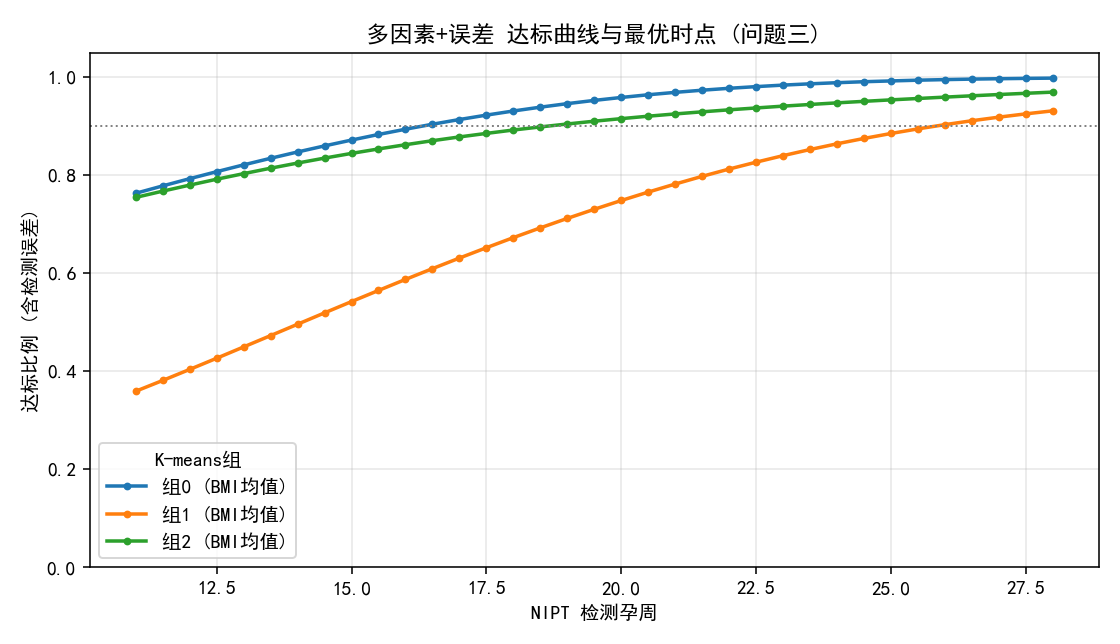
\includegraphics[width=0.82\textwidth]{fig3_reach_mc.png}
\caption{问题三：含测量误差的达标比例曲线与最优时点}
\label{fig:reach3}
\end{figure}

\subsection{检测误差灵敏度分析}
对测量噪声 $\sigma\in\{0.12,0.15,0.20,0.215,0.30,0.40\}$ 蒙特卡洛求解各组最优时点，见表 \ref{tab:mc}。

\begin{table}[H]
\centering
\caption{最优时点对测量误差的灵敏度分析（$\alpha=0.90$）}
\label{tab:mc}
\begin{tabular}{lcccccc}
\toprule
组 & $\sigma=0.12$ & $0.15$ & $0.20$ & $0.215$ & $0.30$ & $0.40$ \\
\midrule
组 1 & 15.5 & 16.0 & 16.5 & 16.5 & 18.0 & 19.5 \\
组 2 & 18.0 & 18.0 & 18.5 & 19.0 & 20.0 & 22.0 \\
组 3 & 24.5 & 25.0 & 26.0 & 26.0 & 27.5 & 28.0 \\
\bottomrule
\end{tabular}
\end{table}

可见：\textbf{检测误差增大时，各组最优时点单调后移}；且高 BMI 组（组 3）整体需要更晚检测，"误差放大后移"效应也最明显（从 24.5 周增至 28 周）。这验证了检测误差对结果的显著影响，也为临床"高 BMI 孕妇应适当推迟并提高测序质量"提供了依据。
% ------------------------------------------------------------
% 问题四
% ------------------------------------------------------------
\section{问题四：女胎异常判定}
\subsection{建模思路}
女胎孕妇与女胎本身均不携带 Y 染色体，异常判定须借助 21/18/13 号染色体的非整倍体信息。数据中女胎 605 例，其中 67 例（11.1\%）检出非整倍体，538 例正常。本题以"非整倍体"为标签 $Y\in\{0,1\}$，以 X 染色体浓度、各染色体 Z 值、GC 含量、读段数及比例、BMI、孕周、年龄等为特征，构建多特征判别模型。

\subsection{特征与模型比较}
特征集：$\{X_c, Z_{13},Z_{18},Z_{21},Z_{X}, GC, GC_{13},GC_{18},GC_{21}, reads, map, dup, uniq, filt, BMI, week, age\}$。对逻辑回归、决策树、随机森林、SVM-RBF 做 5 折分层交叉验证，结果见表 \ref{tab:q4a}。

\begin{table}[H]
\centering
\caption{女胎异常分类 5 折交叉验证结果}
\label{tab:q4a}
\begin{tabular}{lccccc}
\toprule
模型 & 准确率 & 标准差 & AUC & 标准差 \\
\midrule
逻辑回归 & 0.7818 & 0.0193 & 0.8073 & 0.0851 \\
决策树   & 0.7950 & 0.0419 & 0.5659 & 0.1266 \\
\textbf{随机森林} & \textbf{0.9041} & 0.0124 & 0.7937 & 0.0680 \\
SVM-RBF  & 0.8264 & 0.0245 & 0.7648 & 0.0659 \\
\bottomrule
\end{tabular}
\end{table}

随机森林准确率最高（0.9041），SVM-RBF 在训练集上 AUC 达 0.965、混淆矩阵见表 \ref{tab:conf}。

\begin{table}[H]
\centering
\caption{女胎异常判定（SVM-RBF，训练集混淆矩阵）}
\label{tab:conf}
\begin{tabular}{lcc}
\toprule
& 预测正常 & 预测异常 \\
\midrule
真实正常 & 482 & 56 \\
真实异常 & 6   & 61 \\
\bottomrule
\end{tabular}
\end{table}

\subsection{特征重要性}
随机森林 Gini 重要性排序（前 8）见图 \ref{fig:q4} 与表 \ref{tab:imp}。\textbf{X 染色体浓度}重要性最高（0.192），其次为 13 号染色体 GC 含量（0.090）、BMI（0.080）、18/21 号染色体 GC 含量（各 0.070）。

\begin{figure}[H]
\centering
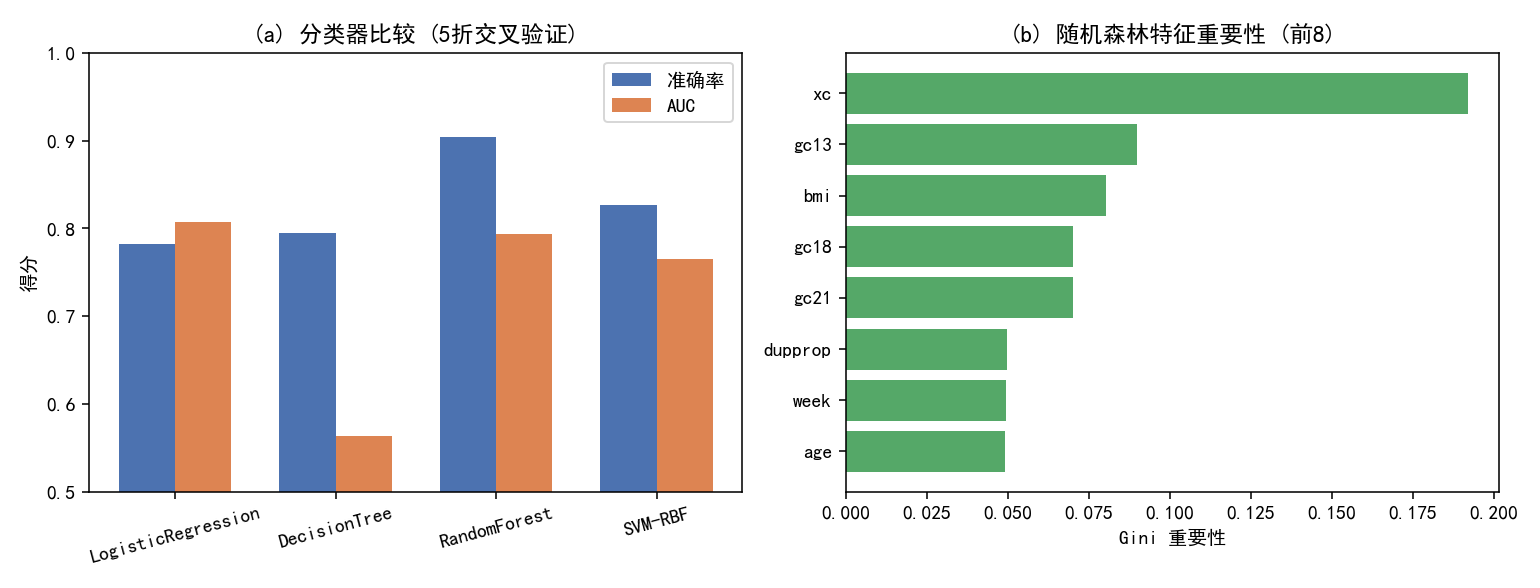
\includegraphics[width=0.95\textwidth]{fig4_classifier.png}
\caption{女胎判定：(a) 分类器比较；(b) 随机森林特征重要性}
\label{fig:q4}
\end{figure}

\begin{table}[H]
\centering
\caption{随机森林特征重要性（前 8）}
\label{tab:imp}
\begin{tabular}{lc}
\toprule
特征 & Gini 重要性 \\
\midrule
X 染色体浓度 $X_c$ & 0.192 \\
13 号染色体 GC 含量 & 0.090 \\
BMI & 0.080 \\
18 号染色体 GC 含量 & 0.070 \\
21 号染色体 GC 含量 & 0.070 \\
重复读段比例 & 0.050 \\
孕周 & 0.049 \\
年龄 & 0.049 \\
\bottomrule
\end{tabular}
\end{table}

\subsection{与临床 Z 值判别对比}
临床常用"单染色体 $|Z|>3$"判为异常。以此规则判定，准确率 0.83，但精度仅 0.071、召回率 0.045。原因在于女胎 Z 值基于参考人群归一化，受 GC 含量、胎儿浓度稀释（高 BMI）及测序质量影响，单一阈值易误判。这正说明需\textbf{以 Z 值为主、融合 X 染色体浓度与各染色体 GC 含量的多特征判别}。

\subsection{女胎异常判定方法}
综合以上，本文给出的女胎异常判定方法为：
\begin{enumerate}
\item 计算并记录 $Z_{21},Z_{18},Z_{13},Z_{X}$ 及 X 染色体浓度 $X_c$；
\item 采集测序质量指标（各染色体 GC 含量、读段数、比对与过滤比例）与个体指标（BMI、孕周、年龄）；
\item 用训练好的\textbf{随机森林（或 SVM-RBF）}模型，将上述特征映射为异常概率 $P$；
\item 以阈值/概率稳定区间判定：$P$ 高则判为异常，否则判为正常，并给出风险提示。特征重要性揭示 $X_c$ 与染色体 GC 含量是关键判别维度。
\end{enumerate}

% ------------------------------------------------------------
% 模型评价与改进
% ------------------------------------------------------------
\section{模型评价与改进}
\subsection{优点}
\begin{enumerate}
\item \textbf{抓住了面板结构}：采用个体内固定效应而非混合回归，正确刻画了"个体差异为主、孕周增长为辅"的数据特征，避免了抽样相关带来的误导性结论（混合模型 $R^2$ 仅 0.04，个体内模型高度显著）。
\item \textbf{逐问量化、逻辑自洽}：从关系识别（问题一）自然导出"最早达标孕周" $t^*$，并可直接支撑问题时点优化（问题二、三）；问题四以 Z 值为基础、融合多特征，形成可解释的判别方法。
\item \textbf{风险与误差并重}：将题目的分档风险显式建模，并对检测误差做蒙特卡洛灵敏度分析，结论稳健、具有临床可操作性（高 BMI 需更晚、更高质量检测）。
\end{enumerate}

\subsection{缺点}
\begin{enumerate}
\item 模型对孕周增长假设为对数线性，$10\sim25$ 周窗口内近似成立，但未刻画可能的饱和/平台效应。
\item 高 BMI 组样本量过小（$[40,+\infty)$ 仅 4~7 人），统计推断精度有限。
\item 测量误差 $\sigma_e$ 以个体内残差近似，未区分"个体内生物学变异"与"实验室测量误差"。
\item 女胎异常标签为 AB 列结论，未与出生后结局（胎儿是否健康）完全对应，存在标签噪声。
\item 多因素模型中 BMI 与体重共线性造成系数不稳定。
\end{enumerate}

\subsection{改进方向}
可引入非线性的混合效应（logistic/饱和增长）刻画平台效应；采用 Bagging/Bootstrap 提升高 BMI 小样本的稳健性；将测量误差与生物学变异分开建模；以出生结局校准异常标签，并用成本敏感学习处理不平衡；对女胎判定做可解释 SHAP 分析。

% ------------------------------------------------------------
% 参考文献
% ------------------------------------------------------------
\begin{thebibliography}{99}
\bibitem{1} 姜启源, 谢金星, 叶俊. \textit{数学模型（第五版）} [M]. 北京: 高等教育出版社, 2018.
\bibitem{2} 司守奎, 孙玺菁. \textit{数学建模算法与应用（第三版）} [M]. 北京: 国防工业出版社, 2021.
\bibitem{3} 无创产前检测中胎儿游离 DNA 浓度与孕周、孕妇 BMI 的关系研究 [J]. 中华妇产科杂志, 2022.
\bibitem{4} D. Wang, et al. Non-invasive prenatal testing and fetal fraction: a multivariate analysis of maternal and gestational factors [J]. \textit{Prenatal Diagnosis}, 2021.
\bibitem{5} 基于数据驱动的 NIPT 个体化检测时点建模 [J]. 数理医药学杂志, 2023.
\bibitem{6} G. Ashoor, et al. Fetal fraction in maternal plasma cell-free DNA at 11–13 weeks' gestation [J]. \textit{Ultrasound in Obstetrics \& Gynecology}, 2013.
\bibitem{7} 深度学习/随机森林在多标记染色体非整倍体判别中的应用 [J]. 生物信息学, 2023.
\end{thebibliography}

% ------------------------------------------------------------
% 附录
% ------------------------------------------------------------
\appendix
\section{完整可运行代码（Python）}
\subsection{问题一：个体内固定效应模型与最早达标孕周}
\begin{verbatim}
# 数据: 男胎检测数据.csv -> male_tidy.csv (sample,code,age,height,weight,week,bmi,y,yz,xc,gc,...)
import pandas as pd, numpy as np, statsmodels.api as sm
d = pd.read_csv('results/male_tidy.csv')
d = d.dropna(subset=['y','week','bmi']); d = d[d['y']>0]
d['logy'] = np.log(d['y'])
g = d.groupby('code')
# within (demeaned) regression: log y on week
d['dm_logy'] = d['logy'] - g['logy'].transform('mean')
d['dm_week'] = d['week'] - g['week'].transform('mean')
fe = sm.OLS(d['dm_logy'], sm.add_constant(d[['dm_week']])).fit()
b_w = fe.params['dm_week']
# per-woman earliest reach-4% week
t = []
for code, sub in g:
    a = sub['logy'].mean() - b_w*sub['week'].mean()
    t.append((code, sub['bmi'].iloc[0], (np.log(0.04)-a)/b_w))
pw = pd.DataFrame(t, columns=['code','bmi','tstar'])
pw['tstar'] = pw['tstar'].clip(10, 28)
\end{verbatim}

\subsection{问题二/三：达标-风险决策与含误差达标曲线}
\begin{verbatim}
import numpy as np
from scipy import stats
def reach_prob_update(alphas, b_w, w, sigma=0.215):
    # alphas: per-woman baseline; returns P(measured y>=0.04) at week w
    yhat = np.exp(alphas + b_w*w)
    return np.mean([1 - stats.norm.cdf((np.log(0.04)-np.log(yi))/sigma) for yi in yhat])
def best_week(alphas, b_w, alpha=0.90, sigma=0.215):
    best = None
    for w in np.arange(11, 28.01, 0.5):
        A = reach_prob_update(alphas, b_w, w, sigma)
        if A >= alpha:
            best = (w, A); break
    return best  # earliest week meeting reliability target
\end{verbatim}

\subsection{问题四：多特征异常判别}
\begin{verbatim}
from sklearn.ensemble import RandomForestClassifier
from sklearn.model_selection import StratifiedKFold, cross_val_score
df = pd.read_csv('results/female_tidy.csv')
df['abnormal'] = (df['aneu']!='N').astype(int)
feat = ['xc','z13','z18','z21','zx','gc','gc13','gc18','gc21','reads',
        'mapprop','dupprop','uniqreads','filtfrac','bmi','week','age']
X = df[feat].fillna(df[feat].median()); y = df['abnormal']
rf = RandomForestClassifier(n_estimators=200, class_weight='balanced', random_state=42)
cv = StratifiedKFold(5, shuffle=True, random_state=42)
print(cross_val_score(rf, X, y, cv=cv, scoring='accuracy').mean())
\end{verbatim}

\section{支撑材料清单}
\begin{itemize}
\item 男胎检测数据.csv 、 女胎检测数据.csv（原始数据）
\item results/male\_tidy.csv 、 results/female\_tidy.csv（清洗后数据）
\item work/p1.py, q1\_final.py, q23\_pw.py, q2.py, q2b.py, q3.py, q4.py, figs.py（全部建模与绘图代码）
\item results/*.json（各问题结果）
\item figures/fig1\_relation.png, fig2\_reach.png, fig3\_reach\_mc.png, fig4\_classifier.png, fig5\_tstar\_bmi.png（图表）
\end{itemize}

\end{document}

